\begin{figure}
    \centering
    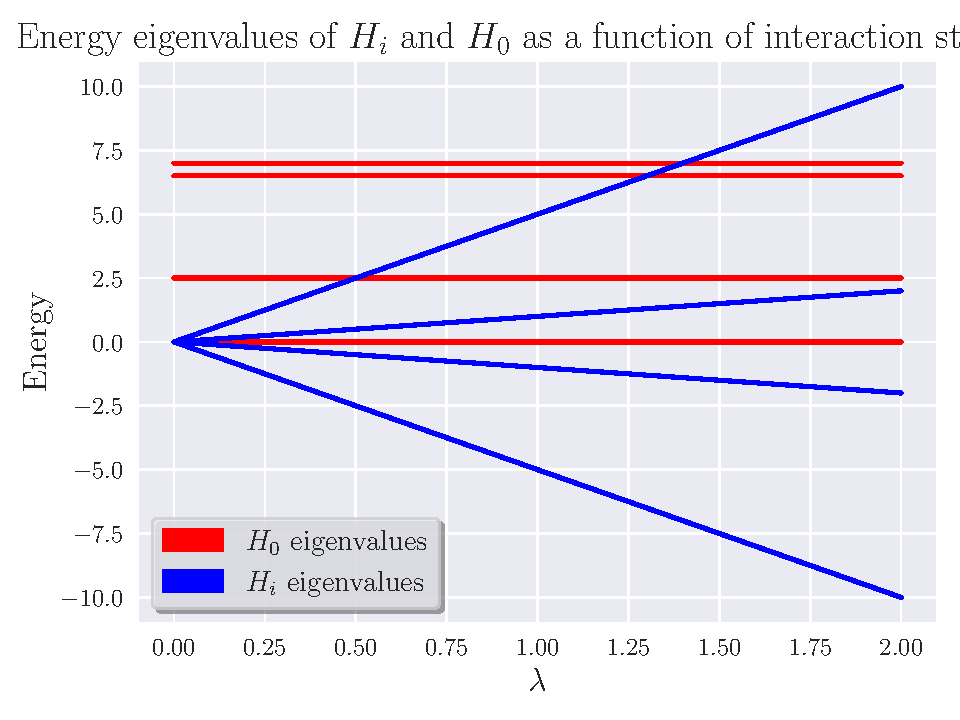
\includegraphics[scale=0.4]{figs/Eig_lmd.pdf}
    \caption{Caption}
    \label{fig:eig_lmd}
\end{figure}
The entropy in Fig. (\ref{fig:entropy}) has an initial contribution which increases slower, before taking a leap for a connection strength of $\lambda \approx 0.4$. This is probably a jump corresponding to a system being slightly interacting into being entangled. The entanglement further increases before converging around $\lambda \approx 1.3$. Studying Fig(\ref{fig:eig_lmd} Overlap) we can extract some information, seeing as the first jump is correlated with the eigenvalues of the interaction Hamiltonian overcoming the second lowest eigenvalues. The convergence can be interpreted as the interaction energy overcoming the higher eigenvalues of the non-interaction Hamiltonian.
\newline\newline

The decision of the ansatz in Fig. (\ref{fig:ansatz}) seems a bit arbitrary, but is based on the ansatz in Hlatshwayo et al. (\cite{hlatshwayoSimulatingExcitedStates2022}). There could be possibilities in optimization by choosing a different ansatz. This would be a section of further research by delving into a review of VQE by Tilly et al. (\cite{VQE_review}). \newline 
Further research could look into other methods of optimization, other than the VQE algorithm, as it is a fairly simple model with restricted applicability. It could probably be extended to solving other optimization problems with minor tweaks or clever encoding. The Lipkin model is fairly limited when it comes to QC. This is a result of the angular momentum operators $j_+$ and $j_-$ are not unitary and thus not applicable to general QC. Thus other models could be further researched in order to not simplify the Hamiltonian by non-unitarity. These models become fairly complex quickly and involves heavier computational costs in order to construct and optimize. \comment{Mangler litt idé om fler ting å kunne ta opp her.} 
